\documentclass[a4paper,11pt]{report}
\usepackage[T1]{fontenc}
\usepackage[utf8]{inputenc}
\usepackage[polish]{babel}
\usepackage{lmodern}
\usepackage{graphicx}

\title{Roznice w czasie odczytu danych z tablicy asocjacyjnej w zależności od implementacji.}
\author{Arkadiusz Cyktor 200367}

\begin{document}
\maketitle


\begin{figure}
  1. Poniższy wykres przedstawia zależność czasu potrzebnego na odczytanie całej zawartości tablicy asocjacyjnej w zależności od ilości danych.
   Linia czerwona odpowiada implementacji przy użyciu drzewa binarnego, zielona - tablicy haszującej, natomiast niebieska reprezentuje tablicę asocjacyjną zaimplementowaną przy pomocy klasy vector.
  \\\begin{center} 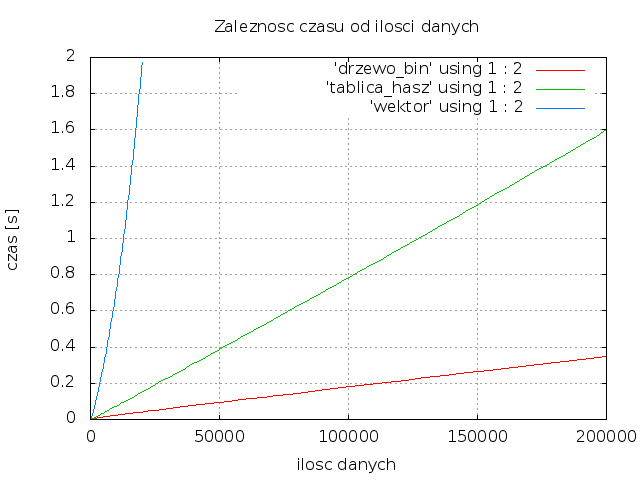
\includegraphics[scale=0.55]{./drzewo_bin+tablica_hasz.png}\end{center}
  Jak widać, wszystkie charakterystyki zmieniają się liniowo, co wydaje się być całkowicie logiczne - im więcej obiektów w tablicy, tym więcej czasu jest potrzebne na ich wypisanie. Implementacje różnią się jednak znacząco tempem wzrostu złożoności.
\\Najwydajniejszym rozwiązaniem okazało się być drzewo binarne - charakteryzuje się ono najmniejszym czasem odczytu.
\\Po środku, znajduje się tablica haszująca, a najgorzej sprawdziła się implementacja wektorowa - pomimo zastosowania sortowania algorytmem quicksort i wyszukiwania binarnego wypada ona niezwykle słabo na tle pozostałych.
\\Należy jednak pamiętać, że mierzone były jedynie czasy odczytów danych z tablicy, w przypadku zapisu wyniki mogą się różnić, wyniki będą również inne, jeśli zmierzymy czas dostępu do jednego, konkretnego elementu, co zostało przedstawione w następnym punkcie.
\end{figure}

\begin{figure}
  \begin{center}
  Tabela z wynikami pomiarów:\\
  \begin{tabular}{|c|c|c|c|}
  \hline 
  Ilość elementów & Czas - drzewo binarne & Czas - tablica haszującac & Czas - wektor\\
  \hline
  100 & 0 & 0 & 0\\
  \hline
  1000	&	0.01 & 0 & 0.01\\
  \hline
  10000	&	0.03 & 0.08 & 0.54 \\
  \hline
  100000 &	0.18 & 0.76 & 1.17\\
  \hline
  200000 &	1.7 & 1.6 & 1.97\\
  \hline
\end{tabular} 
\end{center}
\end{figure}
\begin{figure}
  2. Poniższy wykres przedstawia zależność czasu potrzebnego na odczytanie konkretnego elementu w tablicy asocjacyjnej w zależności od ilości danych. Linia czerwona odpowiada implementacji przy użyciu drzewa binarnego, zielona - tablicy haszującej, natomiast niebieska reprezentuje tablicę asocjacyjną zaimplementowaną przy pomocy klasy vector.
  \\\begin{center} 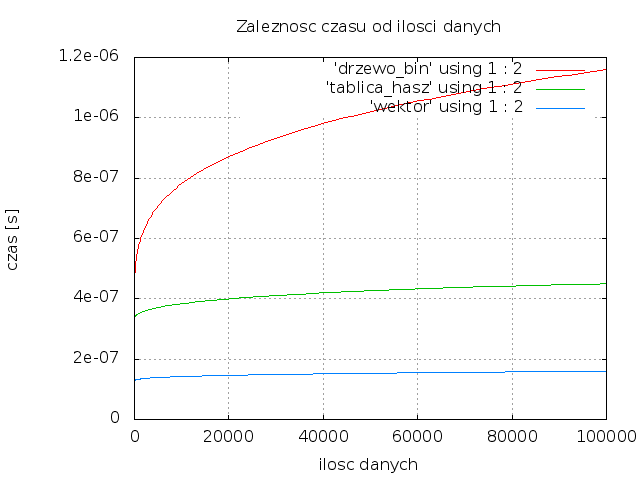
\includegraphics[scale=0.50]{./razem2.png}\end{center}
\end{figure}
\begin{figure}
 \begin{center}
  Tabela z wynikami pomiarów:\\
  \begin{tabular}{|c|c|c|c|}
  \hline 
  Ilość elementów & Czas - drzewo binarne & Czas - tablica haszującac & Czas - wektor\\
  \hline
  100 & 0.00000048 & 0.00000034 & 0.00000013\\
  \hline
  1000	&	0.00000075 & 0.00000037 & 0.00000014\\
  \hline
  10000	&	0.00000096 & 0.00000042 & 0.00000015 \\
  \hline
  100000 &	0.00000116 & 0.00000045 & 0.00000016\\
  \hline

\end{tabular} 
\end{center}
  Jak widać, wyniki uzyskane w tym teście różnią się od poprzednich - tym razem najwydajniejszym rozwiązaniem okazała się być tablica haszująca, która zapewnia w przybliżeniu stały czas dostępu do zawartych w niej elementów, gorzej wypadło drzewo binarne, dla którego zależność czasu od ilości danych kształtuje się logarytmicznie. Oba te rozwiązania zostawiły jednak daleko w tyle implementację tablicy asocjacyjnej przy pomocy klasy vector, ponieważ dostęp do jej ostatniego elementu (a taki wariant był sprawdzany podczas testów) wiąże się z przeszukaniem całejtablicy, to czas realizacji takiej operacji znacząco rośnie wraz ze zwiększającą się ilością danych. 
\\Pomimo jasno widocznej wyższości tablicy haszującej nad innymi testowanymi rozwiązaniami należy pamiętać, że czas dostępu do jej elementów nie zawsze będzie stały - jeśli postanowimy wypełnić ją większą ilością danych niż posiada ona pól, wtedy dojdzie do kolizji, które spowodują przypisanie kilu elementów pod jednym adresem, a to może znacznie wydłużyć czas wyszukiwania.
\end{figure}

\end{document}